\documentclass[a4paper]{article}

\usepackage[a4paper,margin=25mm]{geometry}
\usepackage[english]{babel}
\usepackage{titlecaps}
\usepackage{enumitem}

\Addlcwords{a an the and but for or nor as at by for in of on per to via vs off up out}

\usepackage{parskip} 
\usepackage[T1]{fontenc}
\usepackage{microtype}
\usepackage{setspace}
\setstretch{1.2}


\usepackage{mathtools, amssymb}
\renewcommand{\Vec}[1]{\boldsymbol{#1}}
\let\oldhat\hat
\renewcommand{\hat}[1]{\oldhat{\mathbf{#1}}}

\usepackage{fourier}

\usepackage[dvipsnames]{xcolor}
\definecolor{AUblue}{RGB}{0,61,115}
\definecolor{AUblueDark}{RGB}{0,37,70}


\usepackage{graphicx}
\graphicspath{{./figures/}}
\usepackage{tikz}
\usetikzlibrary{calc, arrows.meta}

\usepackage{enumitem}
\setlist{topsep=4pt,itemsep=2pt,parsep=0pt}
\setlist[enumerate]{label=\alph*)}

\usepackage{siunitx}
\sisetup{
  exponent-product = \cdot,
  output-decimal-marker = {,},
  per-mode = fraction,
}

%Giles Castelles incfig
\usepackage{import}
\usepackage{xifthen}
\usepackage{pdfpages}
\usepackage{transparent}

\newcommand{\incfig}[2][1]{%
  \def\svgwidth{#1\columnwidth}
  \import{./figures/}{#2.pdf_tex}
}

\usepackage{fancyhdr}
\pagestyle{fancy}
\fancyhf{}
\renewcommand{\headrule}{\hbox to\headwidth{\color{AUblueDark}\leaders\hrule height 0.6pt\hfill}}
\setlength{\headheight}{20pt}
\fancyhead[L]{\small\ReportTitle}
\fancyhead[R]{\small\TheDate}
\usepackage{lastpage}
\fancyfoot[R]{\small\thepage{} of \pageref{LastPage}}
\fancyfoot[L]{\small\CourseName}

\newcommand{\PdfTitle}{Exam}
\newcommand{\Dept}{Department of Mechanical and Production Engineering}
\newcommand{\Uni}{Aarhus University}
\newcommand{\ReportTitle}{\titlecap{\PdfTitle}}
\newcommand{\CourseName}{Statics \& Strength of Materials}
\newcommand{\CourseNumber}{290221U006}
\newcommand{\Course}{\CourseName{} --- \CourseNumber}
\newcommand{\TheDate}{\today}
\newcommand{\Logo}{figures/AU}


\usepackage{hyperref}
\hypersetup{
  colorlinks=true,
  linkcolor=AUblue,
  citecolor=AUblue,
  urlcolor=AUblue,
  pdftitle={\PdfTitle},
  pdfcreator={pdfTeX + newtx},
}
\usepackage[nameinlink]{cleveref}

\usepackage{chngcntr}
\newcounter{problem}
\renewcommand{\theproblem}{\arabic{problem}}
\counterwithin{figure}{problem}
\counterwithin{table}{problem}
\numberwithin{equation}{problem}
\makeatletter
\providecommand*\theHproblem{\theproblem}
\renewcommand{\theHfigure}{problem.\theHproblem.\arabic{figure}}
\renewcommand{\theHtable}{problem.\theHproblem.\arabic{table}}
\renewcommand{\theHequation}{problem.\theHproblem.\arabic{equation}}
\makeatother

\crefname{problem}{problem}{problems}
\Crefname{problem}{Problem}{Problems}
\crefname{pluralequation}{equations}{equations}
\Crefname{pluralequation}{Equations}{Equations}

\usepackage{caption}
\captionsetup{font=small}

\newenvironment{problem}[1]%
{%
  \par\vspace{0pt}%
  {\large\bfseries\sffamily\color{AUblueDark}%
    Problem #1%
  }%
  \par\vspace{.35\baselineskip}%
}%
{%
  \par\vspace{.6\baselineskip}%
  {\color{AUblueDark}\rule{\linewidth}{0.8pt}}%
  \vspace{.6\baselineskip}\par%
}

\newcommand{\AUheading}[1]{%
  \par\vspace{.4\baselineskip}%
  {\sffamily\bfseries\color{AUblueDark}#1\par}%
  \nobreak%
}

\newenvironment{assumptions}[1][Assumptions]{%
  \AUheading{#1}
  \begin{itemize}[leftmargin=*,nosep]
}{\end{itemize}\par\medskip}

\newenvironment{derivation}[1][Derivation]{%
  \AUheading{#1}
  \begingroup\allowdisplaybreaks
  \setlength{\abovedisplayskip}{6pt}%
  \setlength{\belowdisplayskip}{6pt}%
  \setlength{\abovedisplayshortskip}{4pt}%
  \setlength{\belowdisplayshortskip}{4pt}%
}{\par\endgroup\medskip}

\newcommand{\finalresult}[1]{%
  \vspace{.2\baselineskip}%
  \begin{equation}
    {\color{AUblueDark}\boxed{\displaystyle #1}}
    \tag*{\textsc{\textcolor{AUblueDark}{Result}}}
  \end{equation}
  \newpage
}

\usepackage{environ}
\newlength{\pbfigsep}
\setlength{\pbfigsep}{8mm}

\NewEnviron{problemwithimage}[3][0.38\linewidth]{%
  \begin{problem}{#3}%
    \noindent
    \begin{minipage}[t]{\dimexpr\linewidth-#1-\pbfigsep\relax}
      \vspace{-0.2\baselineskip}\BODY
    \end{minipage}\hfill
    \begin{minipage}[t]{#1}
      \vspace{-\baselineskip}\centering
      \includegraphics[width=\linewidth]{#2}%
    \end{minipage}%
  \end{problem}%
}

\makeatother
\def\@lecture{}%
\newcommand{\lecture}[3]{
  \ifthenelse{\isempty{#3}}{%
    \def\@lecture{Lecture #1}%
  }{%
    \def\@lecture{Lecture #1: #3}%
  }%
  \refstepcounter{section}%
  \phantomsection
  % Typeset like a subsection (no numbering in the heading)
  \subsection*{\makebox[\textwidth][l]{\@lecture \hfill \normalfont\small\textsf{#2}}}
  % Add a section-level TOC entry with the section number
  \addcontentsline{toc}{section}{\protect\numberline{\thesection}\@lecture}%
}

\makeatletter

\newcommand{\exercise}[1]{%
 \def\@exercise{#1}%
 \subsection{Exercise #1}
}

\newcommand\hr{
  \noindent\rule[1ex]{\linewidth}{0.5pt}
}

\makeatother

\begin{document}
\begin{titlepage}
\thispagestyle{empty}
\onehalfspacing

\begin{tikzpicture}[remember picture,overlay]
  \fill[AUblue] ([xshift=-8mm]current page.west |- current page.north)
       rectangle ([xshift=7mm]current page.west |- current page.south);
\end{tikzpicture}

\vspace*{8mm}
{\large\bfseries \Dept}\\[2pt]
{\normalsize \Uni}
\hfill

\vspace{28mm}
{\fontsize{30pt}{32pt}\selectfont\bfseries \ReportTitle\par}
\vspace{12mm}
{\color{AUblueDark}\rule{\linewidth}{1.5pt}}

\vspace{10mm}
\begin{tabular}{@{}ll}
\textbf{Course:}     & \Course \\
\textbf{Date:}       & \TheDate \\
\end{tabular}

\begin{tikzpicture}[remember picture,overlay]
  \node[anchor=south east, inner sep=0] at
    ($ (current page.south east) + (-20mm, 20mm) $)
    {\includegraphics[width=42mm]{\Logo}};
\end{tikzpicture}

\vfill
\end{titlepage}
    \newpage

    \begin{problem}{1}
      Consider the situation shown in Fig. 1a, where a square plate (in yellow) is connected to a wall via a ball and socket joint at point $A$ and by a smooth support at point $B$.
      The ball and socket joint prevents translation in all directions, whereas the smooth support prevents translation along the negative $y$ axis.
      To maintain equilibrium, the plate is also connected to two cables at points $C$ and $D$.
      The thickness of the plate can be assumed uniform and negligible in relation to the other geometrical dimensions.
      Therefore, points $A$, $B$, $C$, and $D$ can be considered to all lie on the $x$-$z$ plane.

      A composite body is placed on the plate.
      The body consists of a square block and a cylinder placed on top of each other.
      The block, shown in dark blue in Fig. 1b, is made of steel and has section measuring \qty{1}{\m} x \qty{1}{\m} and a height of \qty{0,5}{\m}.
      The cylinder, shown in light blue, is made of glass and has a diameter of \qty{0,4}{\m} and a height of \qty{0,8}{\m}.
      The centroids of the block and the cylinder lie on an axis parallel to the $y$ axis, which intersects the center of the plate.

      \begin{itemize}
        \item[Q1.1] Determine the coordinates of the center of gravity of the composite body, assuming densities of \qty{8000}{\kg\per\m^3} for steel and \qty{2000}{\kg\per\m^3}  for glass.
        \item[Q1.2] Draw a free-body diagram of the plate indicating all the forces acting on it.
        \item[Q1.3] Compute the unit vectors along which the tensions $T_1$ and $T_2$ from the cables connected at points $C$ and $D$ act.
          Express the unit vectors in Cartesian form.
        \item[Q1.4] Use the equilibrium equations to find the magnitude of $T_1$, $T_2$ and all the other reaction forces acting on the plate.
      \end{itemize}
      \begin{figure} [ht]
        \centering
        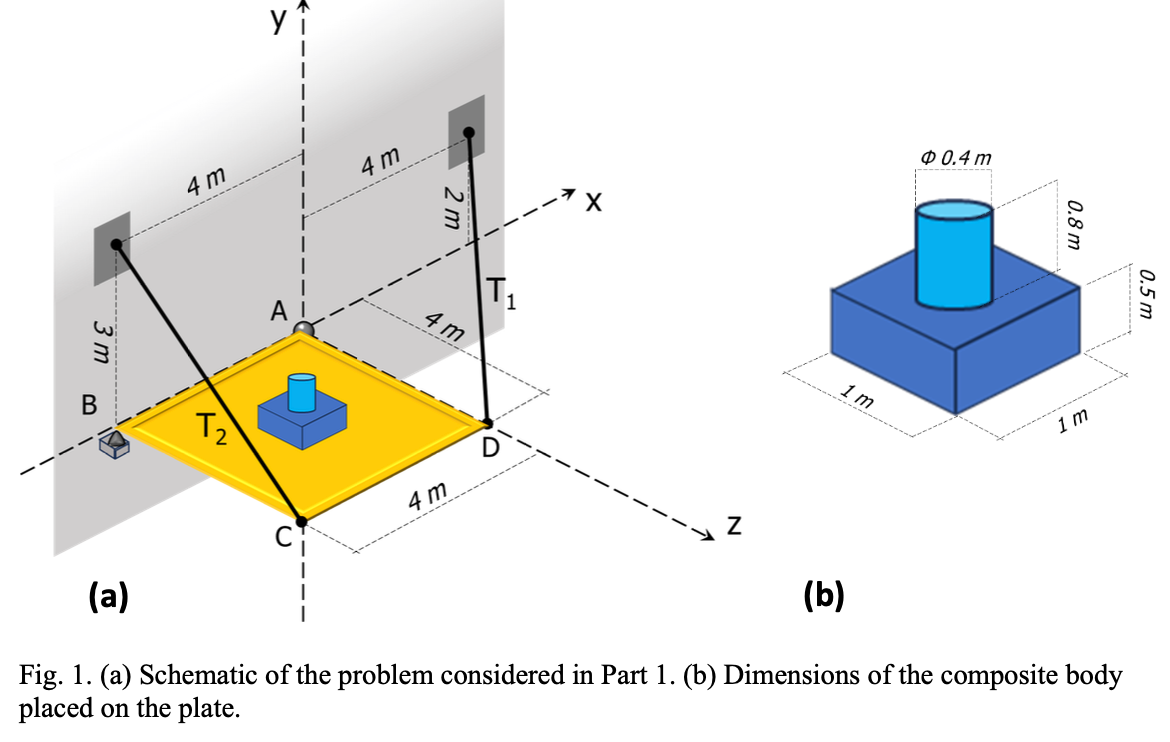
\includegraphics[width=0.8\linewidth]{./figures/e20251.png}
      \end{figure}
    \end{problem}

    \begin{derivation}
      \begin{itemize}
        \item[Q1.1] In the $xz$ plane, the center of gravity of the two parts of the composite body and the plate all lie at $(\overline{x};\overline{z}) = (-2; 2) \, \unit{\m}$. In the $y$ direction the centroid of the composite body can be found using:
          \begin{equation*}
            \overline{y} = \frac{\sum \overline{y}_i \cdot m_i}{m}
          .\end{equation*}
          Where $\overline{y}_i$ is the centroid location in the $y$ direction of one of the parts of the composite body and $m_i$ is the mass of one part of the composite body whilst $m$ is the mass of the entire composite body.
          Hence,
          \begin{align*}
            V_{\mathrm{cyl}} &= \pi \cdot \frac{\left( \qty{0.4}{\m}  \right)^2}{4} \cdot \qty{0.8}{\m}  = \qty{0,1}{\m^3}  \\
            V_{block} &= \qty{1}{\m} \cdot \qty{1}{\m} \cdot \qty{0,5}{\m} = \qty{0,5}{\m^3}  \\
            m_{\mathrm{cyl}} &= \qty{0,1}{\m^3} \cdot \qty{2000}{\kg\per\m^3} = \qty{200}{\kg}  \\
            m_{\mathrm{block}} &= \qty{0,5}{\m^3} \cdot \qty{8000}{\kg\per\m^3} = \qty{4000}{\kg}   \\
            \overline{y} &= \frac{\qty{0.25}{\m} \cdot \qty{4000}{\kg} + \qty{0,9}{\m} \cdot \qty{200}{\kg} }{\qty{4200}{\kg} } = \qty{0,28}{\m}
          .\end{align*}
          This means the coordinates of the center of gravity of the composity body are at:
          \begin{equation*}
            \left( \overline{x}; \overline{y}; \overline{z} \right) = (-2; \num{0,28}; 2)\, \unit{\m}
          .\end{equation*}
        \item[Q1.2] A free-body diagram is shown on \Cref{fig:e20251fbd}. Here, we used the fact that $A$ inhibits motion in all three axes whilst $B$ only inhibits motion in the $y$ axis.
          Furthermore:
          \begin{equation*}
            W = mg = \qty{4200}{\kg} \cdot \qty{9,82}{\m\per\s^2} = \qty{41,244}{\kN}  
          .\end{equation*}
          
        \begin{figure}[ht]
            \centering
            \incfig{e20251fbd}
            \caption{Free body diagram indicating the applied weight $W$ and all reaction components and tension components.}
            \label{fig:e20251fbd}
        \end{figure}
      \item[Q1.3] We start by defining a vector from $C$ to the point on the wall at which $T_2$ is fastened. I.e.
        \begin{equation*}
          \Vec{C}_{\mathrm{wall}} = \qty{0}{\m} \Vec{i} + \qty{3}{\m} \Vec{j} - \qty{4}{\m} \Vec{k}
        .\end{equation*}
        To transform this into a unit vector we must divide it by its length:
        \begin{align*}
          \Vec{u}_{T_2} &= \frac{\Vec{C}_{\mathrm{wall}}}{\left| \Vec{C}_{\mathrm{wall}} \right|} \\
          &= \frac{\qty{3}{\m} \Vec{j} - \qty{4}{\m} \Vec{k}}{\sqrt{\left( \qty{3}{\m}  \right)^2 + \left( \qty{4}{\m}  \right)^2}} \\
          &= \num{0,6} \Vec{j} - \num{0,8} \Vec{k}
        .\end{align*}
        We can follow the same procedure for $T_1$ to get
        \begin{equation*}
          \Vec{D}_{\mathrm{wall}} = \qty{4}{\m} \Vec{i} + \qty{2}{\m} \Vec{j} - \qty{4}{\m} \Vec{k}
        .\end{equation*}
        Which we divide by its length:
        \begin{align*}
          \Vec{u}_{T_1} &= \frac{\Vec{D}_{\mathrm{wall}}}{\left| \Vec{D}_{\mathrm{wall}} \right|} \\
          &= \frac{\qty{4}{\m} \Vec{i} + \qty{2}{\m} \Vec{j} - \qty{4}{\m} \Vec{k}}{\sqrt{\left( \qty{4}{\m}  \right)^2 + \left( \qty{2}{\m}  \right)^2 + \left( \qty{4}{\m}  \right)^2}} \\
          &= \num{0,666} \Vec{i} + \num{0,333} \Vec{j} - \num{0,666} \Vec{k}
        .\end{align*}
        
      \item[Q1.4] A moment equilibrium about point $A$ in the $yz$ plane gives us
        \begin{align*}
          \sum \left( M_A \right)_{yz} &= 0 \\
          T_{2y} \cdot \qty{4}{\m} - W \cdot \qty{2}{\m} + T_{1y} \cdot \qty{4}{\m} &= 0 \\
          T_{1y} + T_{2y} &= \frac{\qty{41,24}{\kN} \cdot \qty{2}{\m} }{\qty{4}{\m} } \\
          T_{1y} + T_{2y} &=\qty{20,62}{\kN} \\
          T_1 \cdot \num{0,333} + T_2 \cdot \num{0,6} &= \qty{20,62}{\kN} 
      .\end{align*}
      And a moment equilibrium about $A$ in the $xz$ plane gives
      \begin{align*}
        \sum \left( M_A \right)_{xz} &= 0 \\
        T_{1x} \cdot \qty{4}{\m} - T_{2z} \cdot \qty{4}{\m} &= 0 \\
        T_{1x} - T_{2z} &= 0 \\
        T_1 \cdot \num{0,666} - T_2 \cdot \num{0,8} &= 0 \\
        T_1 &= \frac{T_2 \cdot (\num{0,8})}{\num{0,666}}  =  \num{1,2} T_2
      .\end{align*}
      Inserting this into our result from the moment equilibrium above we get:
      \begin{align*}
         \num{1,2} T_2 \cdot \num{0,333} + T_2 \cdot \num{0,6} &= \qty{20,62}{\kN}  \\
        T_2 &= \frac{\qty{20,62}{\kN}}{\left( \num{0,6} + \num{1,2} \cdot \num{0,333}  \right)} \\
        T_2 &= \qty{20,62}{\kN} 
      .\end{align*}
      So
      \begin{equation*}
        T_1 = \num{1,2} T_2 = \num{1,2} \cdot \qty{20,62}{\kN} = \qty{24,74}{\kN} 
      .\end{equation*}
      So our tensions are:
      \begin{align*}
        T_1 &= \qty{24,74}{\kN}  \\
        T_2 &= \qty{20,62}{\kN}
      .\end{align*}
      A force equilibrium in the $x$ direction allows us to find $A_x$ as
      \begin{align*}
        \sum F_x &= 0 \\
        A_x + T_{1x} &= 0 \\
        A_x &= - T_{1x} \\
        A_x &= - \qty{24,74}{\kN} \cdot  \num{0,666} = \qty{-16,49}{\kN} 
      .\end{align*}
      A force equilibrium in the $z$ direction gives us:
      \begin{align*}
        \sum F_z &= 0 \\
        A_z - T_{1z} - T_{2z} &= 0 \\
        A_z &= T_{1z} + T_{2z} \\
        A_z &= \qty{24,74}{\kN} \cdot \num{0,666} + \qty{20,62}{\kN} \cdot \num{0,8} \\
        A_z &= \qty{32,99}{\kN} 
      .\end{align*}
      And a force equilibrium in the $y$ direction gives us:
      \begin{align*}
        \sum F_y &= 0 \\
        A_y + B_y + T_{1y} + T_{2y} - W &= 0 \\
        A_y + B_y &= W - T_{1y} - T_{2y} \\
        A_y + B_y &= \qty{41,24}{\kN} - \qty{24,74}{\kN} \cdot \num{0,333} - \qty{20,62}{\kN} \cdot \num{0,6}  \\
        A_y + B_y &= \qty{20,62}{\kN}
      .\end{align*}
      A moment equilibrium about point $A$ in the $xy$ plane gives us
      \begin{align*}
        \sum \left( M_A \right)_{xy} &= 0 \\
        - B_y \cdot \qty{4}{\m} - T_{2y} \cdot \qty{4}{\m} + W \cdot \qty{2}{\m} &= 0 \\
        B_y &= \frac{\qty{41,24}{\kN}  \cdot \qty{2}{\m} - \qty{20,62}{\kN} \cdot \num{0,6} \cdot \qty{2}{\m} }{\qty{4}{\m}} \\
        B_y &= \qty{14,43}{\kN}
      .\end{align*}
      So
      \begin{equation*}
        A_y = \qty{20,62}{\kN} - \qty{14,43}{\kN } = \qty{6,19}{\kN} 
      .\end{equation*}
    \end{itemize}
    \end{derivation}

    \finalresult{
      \begin{aligned}
        &\mathrm{Q1.1} & (\overline{x}; \overline{y}; \overline{z}) &= \left( -2;  \num{0,28}; 2 \right) \, \unit{\m} \\
        &\mathrm{Q1.2} & &\text{See \Cref{fig:e20251fbd}}. \\
        &\mathrm{Q1.3} & \Vec{u}_{T_1} &= \num{0,666} \Vec{i} + \num{0,333} \Vec{j} - \num{0,666} \Vec{k}  \\
        && \Vec{u}_{T_2} &= \num{0,6} \Vec{j} - \num{0,8} \Vec{k} \\
        &\mathrm{Q1.4} & T_1 &= \qty{24,74}{\kN} \quad T_2 = \qty{20,62}{\kN}  \\
        && A_x &= - \qty{16,49}{\kN}  \quad A_y = \qty{6,19}{\kN}  \\
        && A_z &= \qty{32,99}{\kN}  \quad B_y = \qty{14,43}{\kN}
      .\end{aligned}
    }

    \begin{problem}{2}
      Consider a steel T-section cantilever beam loaded as shown in Fig. 2.

      Let $L = \qty{3}{\m}$, $l = \qty{1}{\m}$, $w_0 = \qty{0,5}{\kN\per\m}$, $F_0 = \qty{3}{\kN}$, $E = \qty{200}{\GPa}$, $t = \qty{10}{\mm}$, $f = \qty{25}{\mm}$, $b = \qty{100}{\mm}$, $h = \qty{300}{\mm} $.

      \begin{itemize}
        \item[Q2.1] List all kinematic constraints (boundary conditions) and the associated reactions, determine the degree of static indeterminacy and compute the reaction forces.
        \item[Q2.2] Plot the shear force and bending moment diagrams.
        \item[Q2.3] At the cross section located at $x = L / 2$, determine the state of stress at point $C$ and compute the absolute maximum shear stress (hint: draw the three Mohr circles at point $M$)
        \item[Q2.4] Determine the elastic curve (derive an expression for the beam deflection); in particular, compute the deflection at point $C$.
      \end{itemize}
      The fixed support is now replaced by a pin support, and a column is added below the beam, connected by a pin at point $B$.
      The column is a circular cylinder of radius $R$, length $l$ and is made of the same material as the beam.
      \begin{itemize}
        \item[Q2.5] Assuming a safety factor of \num{1.5}, find the minimum radius $R$, of the column required to prevent buckling while it supports the beam.
      \end{itemize}

      \begin{figure} [ht]
        \centering
        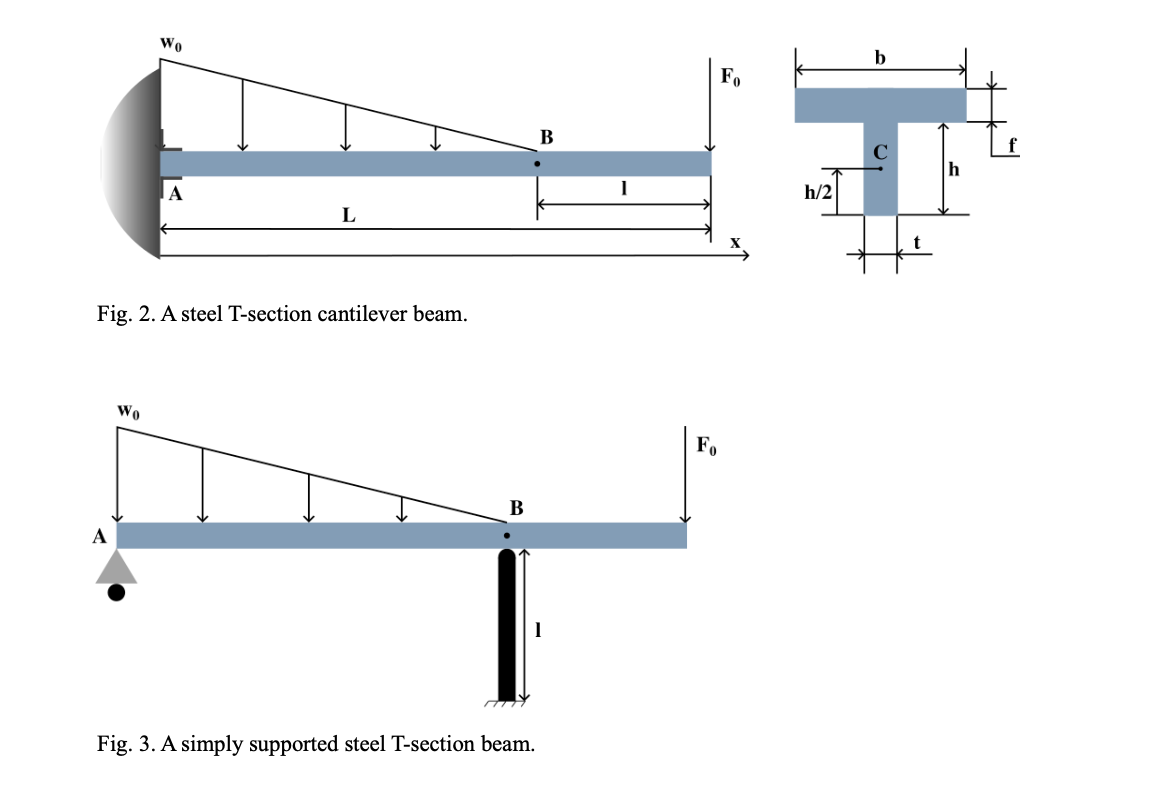
\includegraphics[width=0.8\linewidth]{./figures/e20252.png}
      \end{figure}
    \end{problem}

    \begin{derivation}
      \begin{itemize}
        \item[Q2.1] For the structure, which is a cantilever beam fixed at $A$ we have that transverse deflection and rotation are fixed, $v(0) = 0$ and $v'(0) = 0$.
          At the free end no external moment is applied, so the internal bending moment here must be zero, $M(L) = 0$.
          As we have an applied shear here, the internal shear at the end must be $V(L) = F_0$.
          This means we have three unknown reactions, $A_x$, $A_y$ and $M_0$ and three equilibrium equations $\sum F_x = 0$, $\sum F_y = 0$, $\sum M =0$ which means the structure is determinate. 
        \item[Q2.2] The distributed load corresponds to a point load of
          \begin{equation*}
            W = w_0 \cdot (L-l) \cdot \frac{1}{2} = \qty{0.5}{\kN\per\m} \cdot \qty{2}{\m} \cdot \frac{1}{2} = \qty{0,5}{\kN} 
          .\end{equation*}
          Which acts at a 1/3 of the distance $L-l$, i.e.
          \begin{equation*}
            x_W = \frac{1}{3} \cdot (L-l) = \qty{0,666}{\m} 
          .\end{equation*}
          Using a force equilibrium in the $y$ direction we obtain the reaction $A_y$ at the wall as
          \begin{align*}
            \sum F_y &= 0 \\
            A_y - W - F_0 &= 0 \\
            A_y &= W + F_0  \\
            A_y = \qty{0,5}{\kN} \cdot \qty{3}{\kN} = \qty{3,5}{\kN} 
          .\end{align*}
          Therefore our shear diagram will start at $V(0) = \qty{3,5}{\kN}$. Therefore, the shear diagram is given by:
          \begin{equation*}
            V(x) = \begin{cases}
              A_y - \int_{L-l}^{x} w(s) \, \mathrm{d}s & 0 \leq x \leq L-l \\
             A_y + W & L-l \leq x \leq L 
            .\end{cases}
          .\end{equation*}
          We know that $w(s) = \frac{w_0}{2l}(L - l -s)$ so using GeoGebra we can plot the entire shear diagram as shown on \Cref{fig:e20252s}
          \begin{figure} [ht]
            \centering
            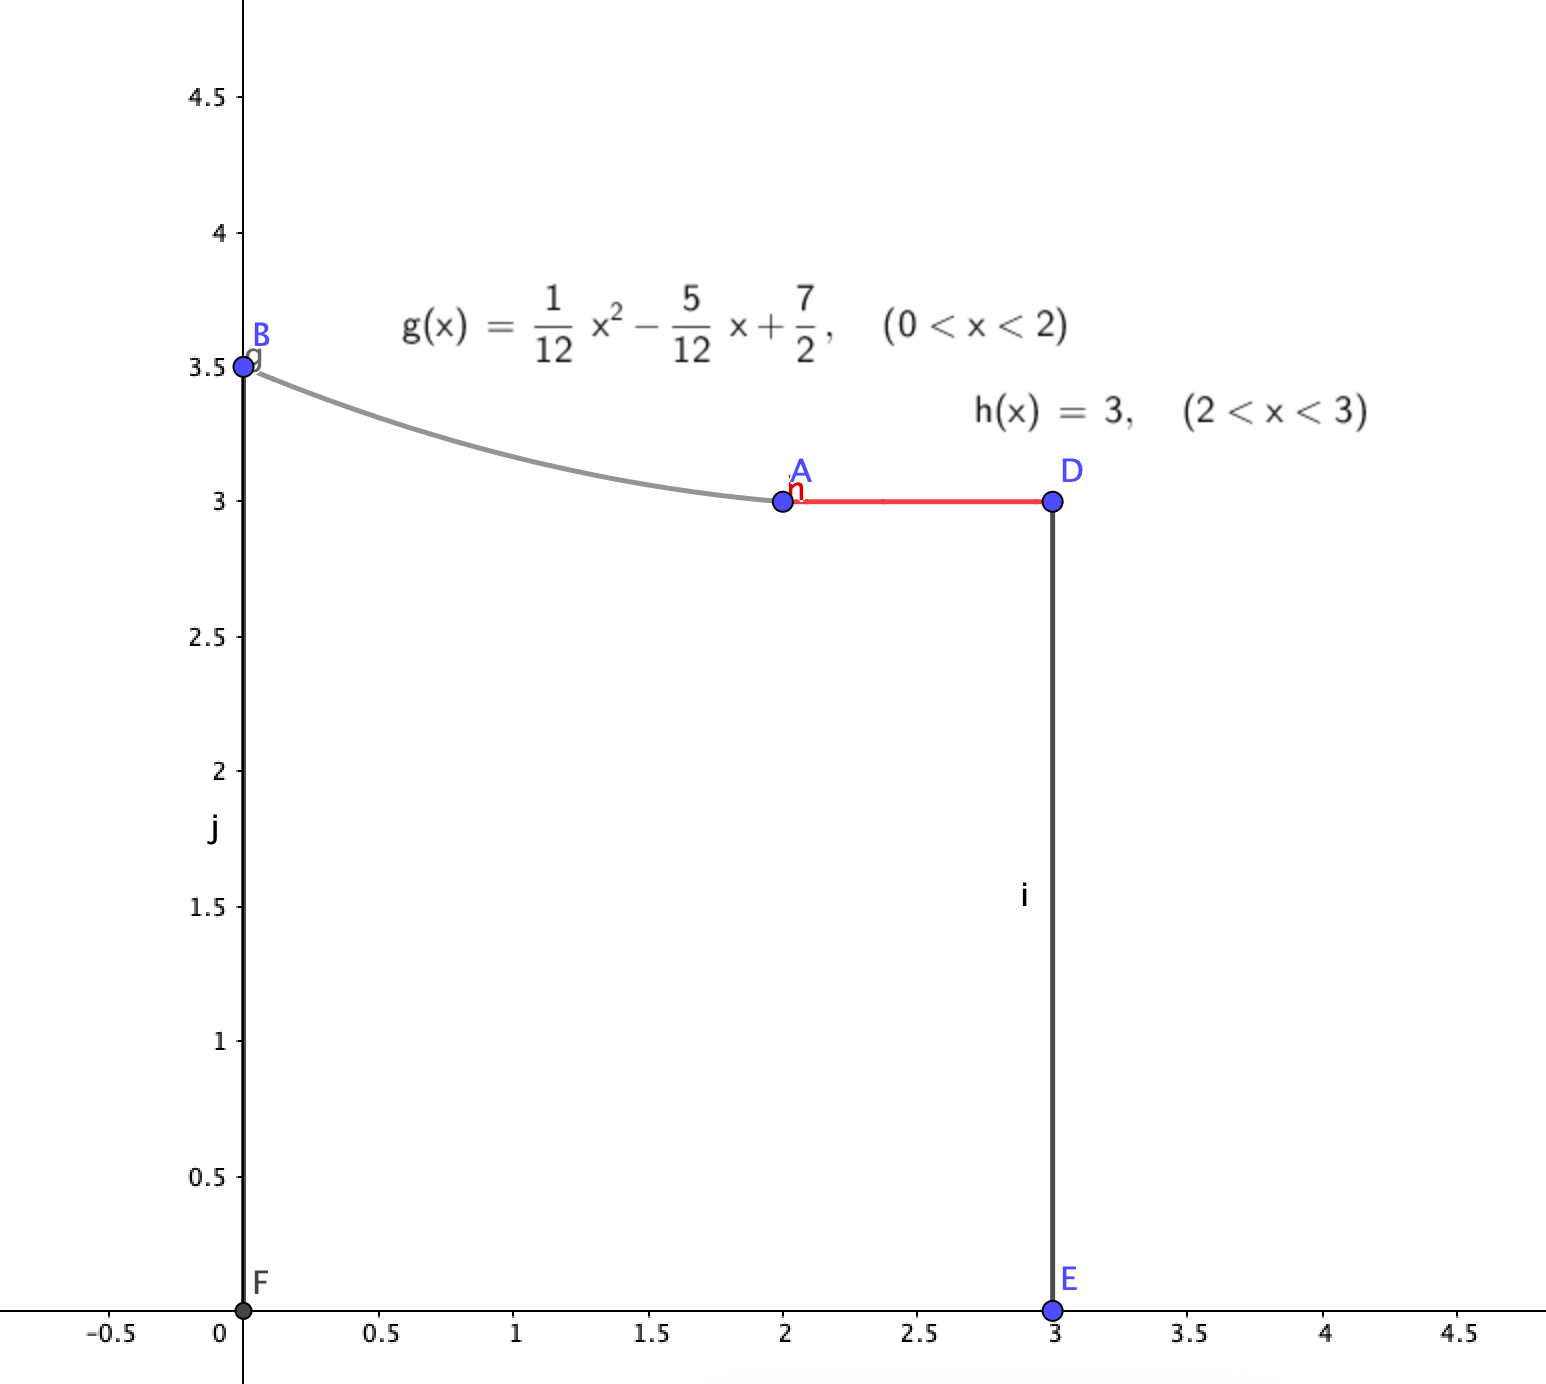
\includegraphics[width=0.5\linewidth]{./figures/e20252s.png}
            \caption{Shear diagram}
            \label{fig:e20252s}
          \end{figure}
          
          From GeoGebra we got the definition
          \begin{equation*}
            V(x) = \begin{cases}
             \frac{1}{12} x^2 - \frac{5}{12} x + \frac{7}{2}  & 0 \leq x \leq L-l\\
             3 & L-l \leq x \leq L 
            .\end{cases}
          .\end{equation*}
          We now use
          \begin{equation*}
            M'(x) = V(x) \implies M(x) = \int V(x) \, \mathrm{d}x 
          .\end{equation*}
          and integrate piecewise to get:
          \begin{equation*}
            M(x) = \frac{1}{36} x^3 - \frac{5}{24} x^2 + \frac{7}{2} x + M_0, 0 \leq x \leq L-l
          .\end{equation*}
          Using a moment equilibrium about point $A$ we can find $M_0$ as:
          \begin{align*}
            \sum M_A &= 0 \\
            M_0 + W \cdot x_W + F_0 \cdot L &= 0 \\
            M_0 &= - W \cdot x_W - F_0 \cdot L \\
            M_0 &=-\qty{0,5}{\kN}\cdot \qty{0,666}{\m} - \qty{3}{\kN} \cdot \qty{3}{\m} \\
            M_0 &= -\qty{9,33}{\kN}
          .\end{align*}
          For the last integration we simply get:
          \begin{equation*}
            M(x) = 3x + C_2, L-l \leq x \leq L
          .\end{equation*}
          For continuity at $x = L-l$ we require
          \begin{align*}
            \frac{1}{36} 8 - \frac{5}{24} 4 + \frac{7}{2} 2  - \num{9,33} &= 3 \cdot 2 + C_2
            C_2 &=  \frac{1}{36} \cdot 8 - \frac{5}{24} \cdot 4 + \frac{7}{2} \cdot 2 - \num{9.33}  - 6 = -8.94111
          .\end{align*}
          Hence,
          \begin{equation*}
            M(x) = \begin{cases}
              \frac{1}{36}x^3 - \frac{5}{24} x^2 + \frac{7}{2}x - \num{9,33} & 0 \leq x \leq 2\\
            3x - \num{8,94} & 2 \leq x \leq 3
            .\end{cases}
          .\end{equation*}
          This is shown on \Cref{fig:e20252m}.

          \begin{figure} [ht]
            \centering
            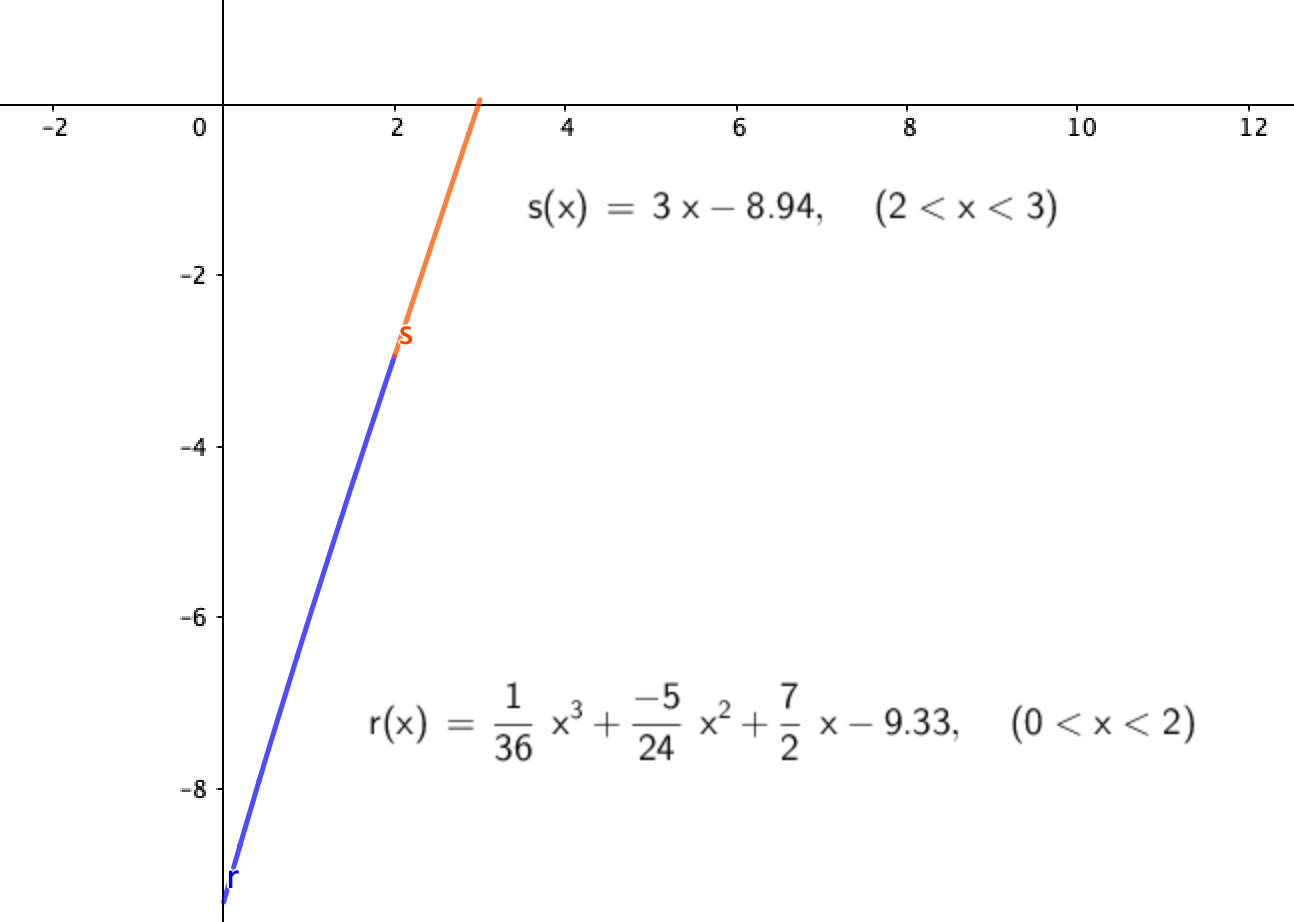
\includegraphics[width=0.5\linewidth]{./figures/e20252m.png}
            \caption{Moment diagram}
            \label{fig:e20252m}
          \end{figure}

        \item[Q2.4] For an Euler-Bernoulli beam, we have that:
          \begin{equation*}
            v''(x) = \frac{M(x)}{EI}
          .\end{equation*}
          Which will be integrated piecewise. For $0 < x < L-l$ we get
          \begin{align*}
            v_1''(x) &= \left( \frac{1}{36}x^3 - \frac{5}{24}x^2 + \frac{7}{2}x - \num{9,33} \right) \cdot \frac{1}{EI} \\
          v_1'(x) &= \frac{\num{0.02778} \left(\frac{x^4}{4}-\num{2,5} x^3+ 63 x^2-\num{335.88} x\right)}{EI} + C_2 \\
          v_1(x) &= \frac{\num{0.001389} x^5-\num{0.0173625} x^4+ \num{0.58338} x^3- \num{4.66537} x^2}{EI} + C_2 x + C_3
        .\end{align*}
        Here we use that $v(0) = 0 \implies C_3 = 0$ and $v'(0) = 0 \implies C_2 = 0$ so
        \begin{equation*}
          v_1(x) = \frac{\num{0.001389} x^5-\num{0.0173625} x^4+ \num{0.58338} x^3- \num{4.66537} x^2}{EI}
        .\end{equation*}
        
        For $L-l < x < L$ we get:
        \begin{align*}
          v_2''(x) &= \frac{3x - \num{8,94} }{EI} \\
          v_2'(x) &= \frac{3 \left(\frac{x^2}{2}- \num{2,98}  x\right)}{EI} + C_4 \\
          v_2(x) &= \frac{\num{0,5}  x^3-\num{4,47}  x^2}{EI} + C_4 x + C_5
        .\end{align*}
        For continuity at $x = L-l$ we require
        \begin{align*}
          v_1'(L-l) &= v_2'(L-l) \\
          v_1(L-l) &= v_2(L-l)
        .\end{align*}
        So:
        \begin{align*}
\frac{\num{0.02778} \left(\frac{(2)^4}{4}-\num{2,5} (2)^3+ 63 (2)^2-\num{335.88} x\right)}{EI} &= \frac{3 \left(\frac{(2)^2}{2}- \num{2,98}  \cdot 2\right)}{EI} + C_4 \\
C_4 &= \frac{\num{0.02778} \left(\frac{(2)^4}{4}-\num{2,5} (2)^3+ 63 (2)^2-\num{335.88} \cdot 2\right)}{EI}  -  \frac{3 \left(\frac{(2)^2}{2}- \num{2,98}  \cdot 2\right)}{EI}  \\
C_4 &= -\frac{\num{0.225413}}{EI}
        .\end{align*}
        and
        \begin{align*}
          \frac{\num{0,5}  2^3-\num{4,47}  2^2}{EI} - \frac{\num{0,225413}}{EI} \cdot 2  + C_5 &= \frac{\num{0.001389} 2^5-\num{0.0173625} 2^4+ \num{0.58338} 2^3- \num{4.66537} 2^2}{EI}  \\
          C_5 &=  \frac{\num{0.001389} 2^5-\num{0.0173625} 2^4+ \num{0.58338} 2^3- \num{4.66537} 2^2}{EI} - \frac{\num{0.52}^3 - \num{4.472}^2 }{EI} + \frac{\num{0.225413}}{EI} \cdot 2\\
           C_5   &= \frac{6.08121}{EI}
        .\end{align*}

        So:
        \begin{equation*}
          v(x) = \begin{cases}
            \frac{\num{0,001389} x^{5} - \num{0,0173625} x^{4} + \num{0.583338} x^3 - \num{4,66537} x^2}{EI} & 0 \leq x \leq L-l\\
            \frac{\num{0,5} x^3 - \num{4,47} x^2}{EI} - \frac{\num{0,225413}}{EI}x + \frac{\num{6,08121}}{EI} & L-l \leq x \leq L
          .\end{cases}
        .\end{equation*}

        This is plotted on \Cref{fig:e20252d}.

        \begin{figure} [ht]
          \centering
          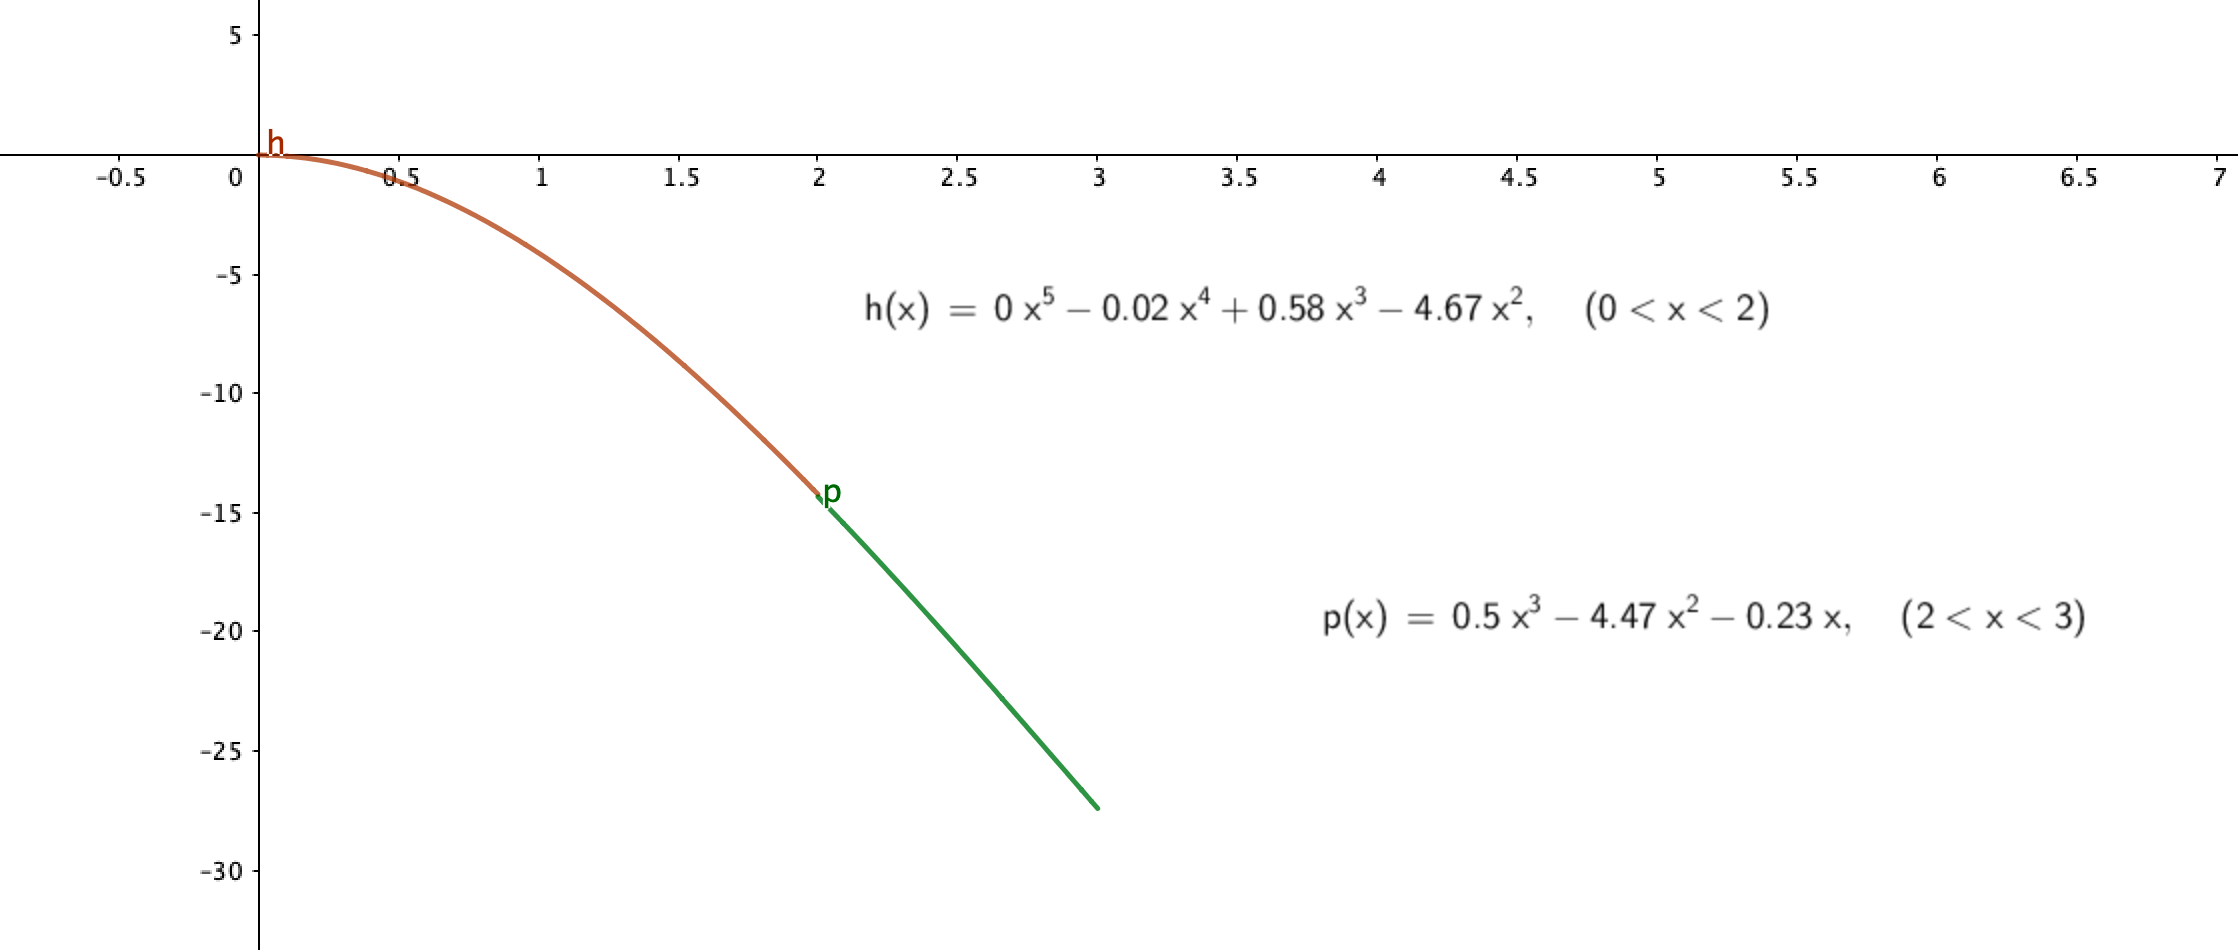
\includegraphics[width=0.5\linewidth]{./figures/e20252d.png}
          \caption{Deflection diagram}
          \label{fig:e20252d}
        \end{figure}
        Using this, the deflection at $C$ is $v(C) = v(L-l) = - \qty{14,33}{\mm}$.

        \item[Q2.5] I do not have time for this part but I would use the formula for critical load:
          \begin{equation*}
            P_{\mathrm{cr}} = \frac{\pi^2 EI}{\left( KL \right)^2}
          .\end{equation*}
          With $K = \num{0,7} $ for a column fixed at the bottom and free at the top.
          I would then solve for the required second moment of area $I$ and find the radius of the smallest circular rod having at least this high a value of $I$.
      \end{itemize}
    \end{derivation}

    \finalresult{
      \begin{aligned}
        &\mathrm{Q2.1} & &\text{See the section}   \\
        &\mathrm{Q2.2} & &\text{See \Cref{fig:e20252s} and \Cref{fig:e20252m}}. \\
        &\mathrm{Q2.3} & \text{No Answer} \\
        &\mathrm{Q2.4} & & \text{See \Cref{fig:e20252d}} \\
        && v(C) &= - \qty{14,33}{\mm} \\
        &\mathrm{Q2.5} & &\text{See the section.}
      .\end{aligned}
    }
\end{document}
